%% LyX 2.3.7 created this file.  For more info, see http://www.lyx.org/.
%% Do not edit unless you really know what you are doing.
\documentclass[english]{article}
\usepackage[T1]{fontenc}
\usepackage[latin9]{inputenc}
\usepackage{babel}
\usepackage{amsmath}
\usepackage{amssymb}
\usepackage{graphicx}
\usepackage[unicode=true]
 {hyperref}
\begin{document}
Suppose you are in a new city and looking to get dinner with friends.
You pull out Google Maps to help with the decision. To make the process
easier, you decide to look at the ratings: A nearby Cambodian restaurant
boasts 4.8 stars, but the equally close Italian place is a close competitor
at 4.6 stars, but has five times the number of reviews. Surely that
must make a difference? You search for your scratchpad, promising
to your friends that you got the situation. 

This is a decision problem with partial information. You suppose that
any restaurant has a true ``overall quality'' that is measurable
in stars. It is what Google Maps would show if all of the world had
visited that place and left a review, call it $r^{\star}$. However,
you have to deal with just a tiny fraction of the reviews and now
have to make sense of it -- an inference. 

No inference without a model. So you assume a couple of things: First,
that reviews are unbiased: The typical review $r$ should be equally
likely to fall above or below the ground truth
\[
\langle r_{i}\rangle=r^{\star}
\]

Moreover, you assume that every reviewer $i$ is off due to their
personal idiosyncracy in assesing restaurants, let's call it
\[
|r_{i}-r^{\star}|=\sigma_{r_{i}}.
\]

To make things easier, you now invoke the central limit theorem 
\[
\frac{1}{N}\sum_{i}^{N}r_{i}\sim\mathcal{N}\Bigl(r^{\star},\,\bigl(\frac{1}{N}\sum_{i}\sigma_{r_{i}}\bigr)^{2}/N\Bigr),
\]

meaning that the empirical average review fluctuates around the true
value $r^{\star}$, typically being off by $\sigma_{r}/\sqrt{N}$,
with $\sigma_{r}=\frac{1}{N}\sum_{i}\sigma_{r_{i}}$ being the average
reliability of the reviewers. From this, we already see that more
reviews drastically help to accurately estimate the quality of a restaurant. 

Now you double down: How likely is the Cambodian place ($C$) indeed
better than the Italian ($I$) one?

\begin{align*}
P\left(r_{C}^{\star}>r_{I}^{\star}\right) & =\int dr_{C}\,dr_{I}P_{C}(r_{C})P_{I}(r_{I})\,\mathbb{I}\left[r_{C}>r_{I}\right]\\
 & =\int\frac{dr_{C}^{\star}}{\sqrt{2\pi\sigma_{r_{C}}^{2}/N_{C}}}\,\int\frac{dr_{I}^{\star}}{\sqrt{2\pi\sigma_{I}^{2}/N_{I}}}\,\exp\left\{ -\frac{\left(\hat{r_{C}^{\star}}-r_{C}^{\star}\right)^{2}}{2\sigma_{r_{C}}^{2}/N_{C}}-\frac{\left(\hat{r_{I}^{\star}}-r_{I}^{\star}\right)^{2}}{2\sigma_{I}^{2}/N_{I}}\right\} \,\mathbb{I}\left[r_{C}^{\star}>r_{I}^{\star}\right].
\end{align*}

Here, $\mathbb{I}$ is an indicator function that is $1$ whenever
its argument is true. 

Unfortunately, this expression does not have a closed form solution.
However, we can readily evaluate the integrand numerically:

\begin{figure}
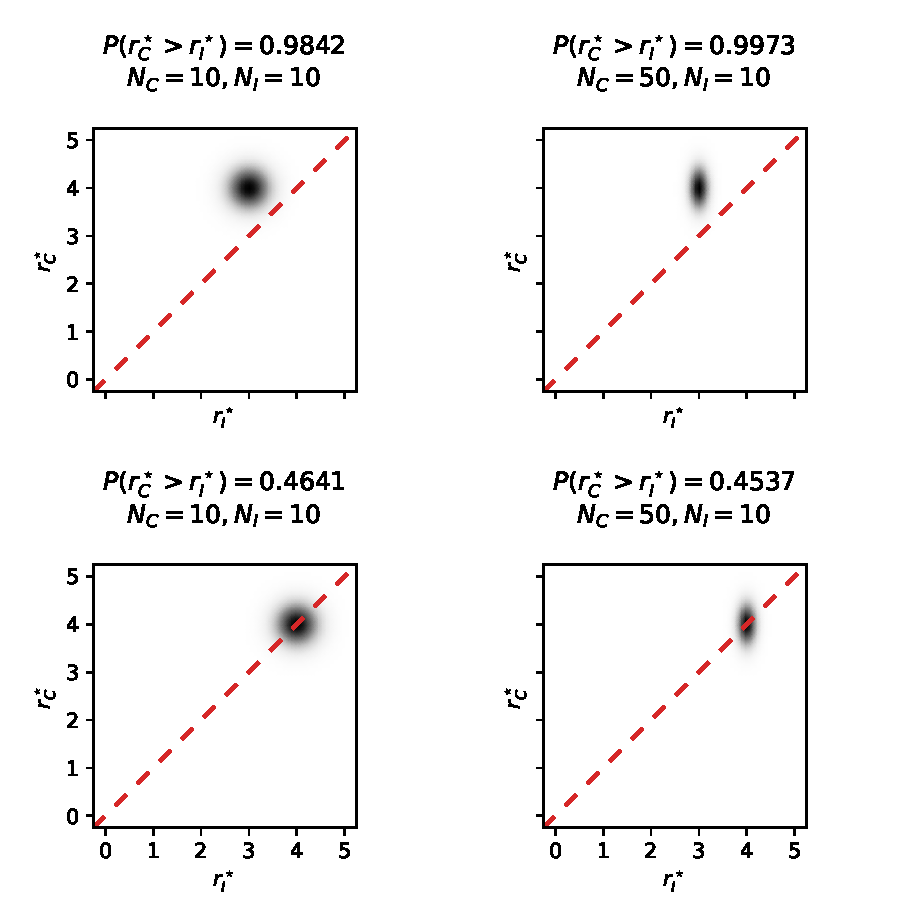
\includegraphics{main}

\caption{}
\end{figure}
In this figure, the two variables are plotted on either axis, and
the condition $\mathbb{I}\left[r_{C}^{\star}>r_{I}^{\star}\right]$
amounts to summing only the upper left diagonal of the space.

\paragraph*{A practical rule}

In case you don't have your laptop with you to make such plots when
you're out, you can use a rule of thumb: Just add the variances $\sigma=\sqrt{\sigma_{r_{C}}/\sqrt{N_{C}}+\sigma_{r_{I}}/\sqrt{N_{I}}}$
. Even simpler, you may add them directly or just choose the maximum
$\sigma=\text{max}\left\{ \sigma_{r_{C}}/\sqrt{N_{C}},\,\sigma_{r_{I}}/\sqrt{N_{I}}\right\} $
if one is much bigger. Now, ask if $\hat{r_{C}^{\star}}>\hat{r_{I}^{\star}}+\sigma$
(or vice versa if the other rating is superior.. If this still holds
true, then you can be approximately 68\% percent sure that the Cambodian
place $C$ is indeed superior. If $\hat{r_{C}^{\star}}>\hat{r_{I}^{\star}}+2\sigma$,
then you can even be about 96\% sure (see \href{https://en.wikipedia.org/wiki/68\%E2\%80\%9395\%E2\%80\%9399.7_rule}{here}
for the rough idea behind that).
\end{document}
